\chapter{Il Corpo Rigido: Spostamenti e Velocit\`a}

\section{Introduzione}

\begin{wrapfigure}{r}{0.5\textwidth}
     \begin{center}
     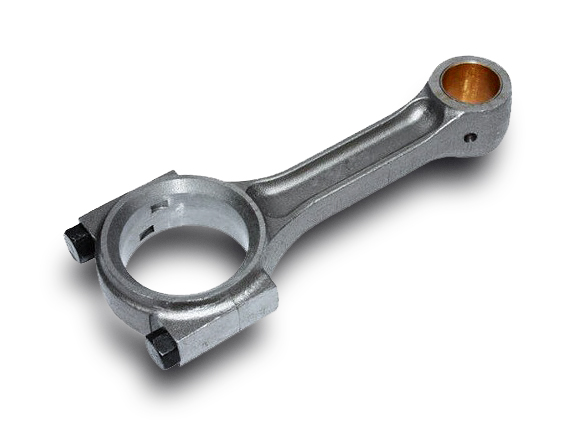
\includegraphics[width=0.42\textwidth]{part1/cinematica/FIG/f11.jpeg}
     \end{center}
\vskip -7.3mm
	\caption{\em Biella di motore d'automobile.}\index{biella}
     \label{fig:f11}
\end{wrapfigure}

Le macchine sono costituite da un certo numero di parti, molte delle
quali 
sono corpi rigidi. {\em Bielle},  \index{biella} {\em manovelle}, \index{manovella}
{\em aste}, {\em bilancieri}, \index{bilanciere}{\em ruote dentate},
\index{ruote!dentate} {\em telai}, \index{telaio} sono tutti {\em corpi rigidi}. 
Per definizione, un corpo \`e rigido \index{corpo rigido} se risulta essere 
invariante nel tempo la distanza tra due suoi punti scelti ad arbitrio. Siano $P_1$ e $P_2$
punti appartenenti al nostro corpo: perch\'e tale corpo sia rigido deve essere
\begin{equation}
	d(P_1, P_2, t_1) = d(P_1, P_2,t_2)\,,
	\label{e11}
\end{equation}
\noindent dove $d(.,.,.)$ \`e la funzione distanza tra due punti al tempo $t$.
Come vedremo tra poco, la
definizione di corpo rigido appena introdotta
risulter\`a essere di grande utilit\`a
nello studio della cinematica, in quanto i corpi rigidi possono dare luogo
esclusivamente a {\em spostamenti rigidi}\footnote{
	Non \`e vero il contrario: anche corpi deformabili come gas e liquidi possono muoversi rigidamente. 
La condizione \ref{e11} fa s\`i che un tetraedro, formato prendendo
come vertici quattro punti qualsiasi del corpo, rimanga invariato
nella forma
anche dopo un eventuale spostamento.
Non \`e difficile immaginare una
bolla d'aria all'interno di un liquido che scorra in
una condotta trasparente (in modo da poter essere osservata), la quale si muova
senza cambiare forma.
}.
\noindent La definizione enunciata poc'anzi ci offre, peraltro, l'opportunit\`a di riflettere sui modelli che mettiamo
in campo per utilit\`a nello studio dei fenomeni naturali: in questo caso
si intuisce che nessun corpo ``reale'' potr\`a
rispettare rigorosamente la \ref{e11},
dato che non esistono corpi indeformabili.
Ma il modello, cio\`e la rappresentazione
ideale e parziale, che si deduce dalla \ref{e11} indica anche la via che si desidera
percorrere nell'indagine scientifica: il corpo rigido \`e utile per
lo studio della cinematica
degli organi delle macchine, dove risulta comodo e appropriato (ma questo si deve verificare 
a posteriori) trascurare le elasticit\`a.
Tale modello non sarebbe affatto opportuno 
qualora il campo di ricerca
fosse quello della resistenza dei materiali, dove gli oggetti considerati sono
posti sotto carico
e subiscono delle variazioni (di norma piccole) della loro forma:
in questo caso il modello del {\em corpo rigido} non
solo sarebbe fuori luogo, ma risulterebbe un 
ostacolo insormontabile nel considerare le deformazioni che subiscono tali corpi.
La biella di un motore endotermico, figura \ref{fig:f11}, sar\`a considerata come un
{\em corpo rigido} nello studio della cinematica dei manovellismi, ma 
nessuno negher\`a che tale biella si deformer\`a sotto gli effetti
del carico laterale dovuto alle sue accelerazioni,
come si studia di fatto
nella disciplina che ha nome {\em Costruzione di Macchine}\footnote{
Questa nota vorrebbe
invitare lo studente a una riflessione circa la natura, 
l'utilit\`a e i limiti dei modelli che si impiegano ai fini di studiare
e di prevedere il comportamento, anche oltre l'immediato
presente, degli oggetti e dei fenomeni
che popolano il mondo circostante. La {\em Teoria dei Modelli}\index{teoria
dei modelli}
\`e una scienza a s\'e stante, dunque questa digressione
non ha alcuna pretesa
di completezza n\'e di profondit\`a.

\noindent Modellare il comportamento di un sistema reale
significa tentare un parallelo tra la realt\`a, complessa e 
ricchissima di dettagli, e altre strutture (i modelli appunto), talvolta
matematiche, altre
volte informatiche, oppure anche esse fisiche che, 
essendo intrinsecamente pi\`u sintetiche e meno doviziose di particolari,
probabilmente inessenziali,
risultano pi\`u comode da indagare e spesso feconde di risultati.
Tali risultati potranno essere considerati validi per il sistema reale soltanto
se confrontabili positivamente
con l'esperienza, nel perimetro
di tutti gli aspetti che nel modello sono stati considerati.
Ad esempio, sembrerebbe strano poter ricavare da un {\em modello urbanistico
fisico},
cio\`e da quelle tavole di legno compensato su cui gli architetti costruiscono
le loro citt\`a in scala ridotta, ricavare, dicevo, informazioni riguardanti
la risposta sismica dei fabbricati; sarebbe impossibile persino scuotendo
energicamente la tavola.

\noindent I modelli matematici e numerici sono ancora pi\`u austeri: fecondi di risultati, semplici
e sicuri, ma intrinsecamente refrattari a essere infarciti di particolari.
Trascurare il colore di un oggetto reale che si modella con il {\em metodo
degli elementi finiti} \`e un comportamento che tutti i tecnici 
approvano, e con ragione. Ma la legittimit\`a di questo comportamento, cio\`e
di trascurare ``arbitrariamente'' nei modelli alcune caratteristiche della
realt\`a, necessita comunque del conforto sperimentale o con modelli di altra
natura.

\noindent I modelli insomma spogliano la realt\`a di molti dettagli e caratteristiche
ritenuti inutili ai fini di prevedere ``ci\`o che accadr\`a'': 
l'impatto urbanistico di un nuovo quartiere o la frequenza delle
oscillazioni del pendolo di una certa lunghezza.
Quanto pi\`u
la realt\`a ``alleggerita'' che si ottiene da un modello
\`e semplice, priva di 
informazioni inessenziali, tanto pi\`u sar\`a
facile interpretarne i risultati,
sempre da verificare, limitatamente all'ambito per il quale il modello \`e stato pensato.
}.

\section{Spostamenti e Velocit\`a}

\noindent {\em Posizione} \index{posizione} e {\em velocit\`a} \index{velocit\`a}
appaiono a chiunque come concetti ampiamente
intuitivi. Del resto siamo abituati a conoscere la velocit\`a
dei nostri spostamenti in automobile semplicemente
leggendo il {\em tachimetro} \index{tachimetro} del cruscotto.
Per quel che riguarda poi la nostra posizione, avvertiamo la sensazione 
che tutto ci\`o che ci circonda funga da {\em sistema di riferimento}
naturale. Sappiamo, in generale, renderci conto senza sforzo della nostra
posizione: ci troviamo a Milano, nella Piazza del Duomo, giusto all'ingresso...
Posizione e velocit\`a sono peraltro a disposizione di tutti gli
utenti di dispositivi dotati di GPS \index{GPS}({\em Global Positioning System}). 

\noindent Qualche difficolt\`a emerge qualora, ad esempio, si volesse conoscere la
velocit\`a del piede di un calciatore nell'istante in cui calcia il pallone.
Tale difficolt\`a nasce dall'intuizione che la velocit\`a del piede del
calciatore
difficilmente coincider\`a con la velocit\`a del calciatore stesso, cio\`e
con quella che potrebbe
essere dedotta da un orologio con GPS indossato dall'atleta.
Allo stesso modo nessuno troverebbe corretto
identificare la velocit\`a delle dita di un pianista durante un concerto
con la velocit\`a del pianista stesso, il quale, di solito, sta seduto su di
uno sgabello.
Eccoci venuti al punto: i corpi, gli oggetti, sono i protagonisti
del movimento ma i concetti 
di {\em spostamento}\index{spostamento} e di {\em velocit\`a}\index{velocit\`a}
si mostrano estremamente adatti a essere applicati a punti precisi di tali oggetti
in movimento. Locuzioni come ``in questo istante
il modulo della velocit\`a della punta dell'indice del
pianista \`e di $0.5 m/s$'' assumono immediatamente carattere 
di indicazione molto accurata, ammesso che la punta dell'indice
sia un riferimento tanto preciso da renderci soddisfatti.
\noindent \`E subito chiaro che,
seguendo la strada sulla quale ci siamo incamminati, non ci accontenteremo
di punta delle dita o di altri riferimenti approssimativi, perci\`o
diremo che
{\em spostamenti} e {\em velocit\`a} appartengono esclusivamente ai punti dei
corpi mobili, e sono pertinenti (ma questo si sapeva gi\`a) soltanto agli
istanti di tempo ai quali vengono riferiti. 
Nel dire tutto questo, il linguaggio della matematica e della geometria
ci pu\`o venire in grande aiuto.
La figura \ref{fig:f12} mostra un {\em corpo rigido} {\bf C} che ha sub\`ito
uno spostamento rigido e {\em piano}.
Quest'ultimo aggettivo aggiunge un'informazione
importantissima e restrittiva: tutti i {\em vettori spostamento} degli infiniti
punti di tale corpo saranno contenuti in piani fra loro paralleli.
Per esempio, limitando la presente introduzione
ai soli {\em moti piani}\index{moti piani}, il concetto di {\em velocit\`a angolare}, che introdurremo
a breve, sar\`a  pi\`u semplice rispetto al caso generale 
di moto rigido tridimensionale, di conseguenza lo sar\`a l'intera trattazione dei
moti piani.
Questa scelta limita non poco la portata del presente lavoro e non sarebbe 
giustificata dalla sola semplificazione dei concetti cinematici
che ne consegue,
se 
la maggior parte dei moti che si verificano nelle macchine non fosse
di questa specie, cio\`e {\em moti piani}.
Si possono comunque rilevare molte eccezioni: le viti di azionamento e di manovra, le
ruote sterzanti (e non) dei veicoli, ecc. Ma i casi pi\`u importanti di moti 
non piani, attinenti la meccanica delle macchine, si verificano
nell'ambito dei {\em robot}.
Vi \`e per\`o da dire che la cinematica tradizionale
che considera i moti
tridimensionali, riportata comunque a grandi linee e in ristrettissimo
compendio nel capitolo \ref{3d},
si mostra piuttosto inefficiente per lo studio della 
{\em Meccanica dei Robot}. Infatti, in quest'ambito \`e d'uopo
 una trattazione algebrica {\em ad hoc},
basata su specifiche matrici $4\times4$, \cite{denavit},
e questo ci fa sentire meno in colpa.
\begin{wrapfigure}{r}{0.45\textwidth}
      \begin{center}
      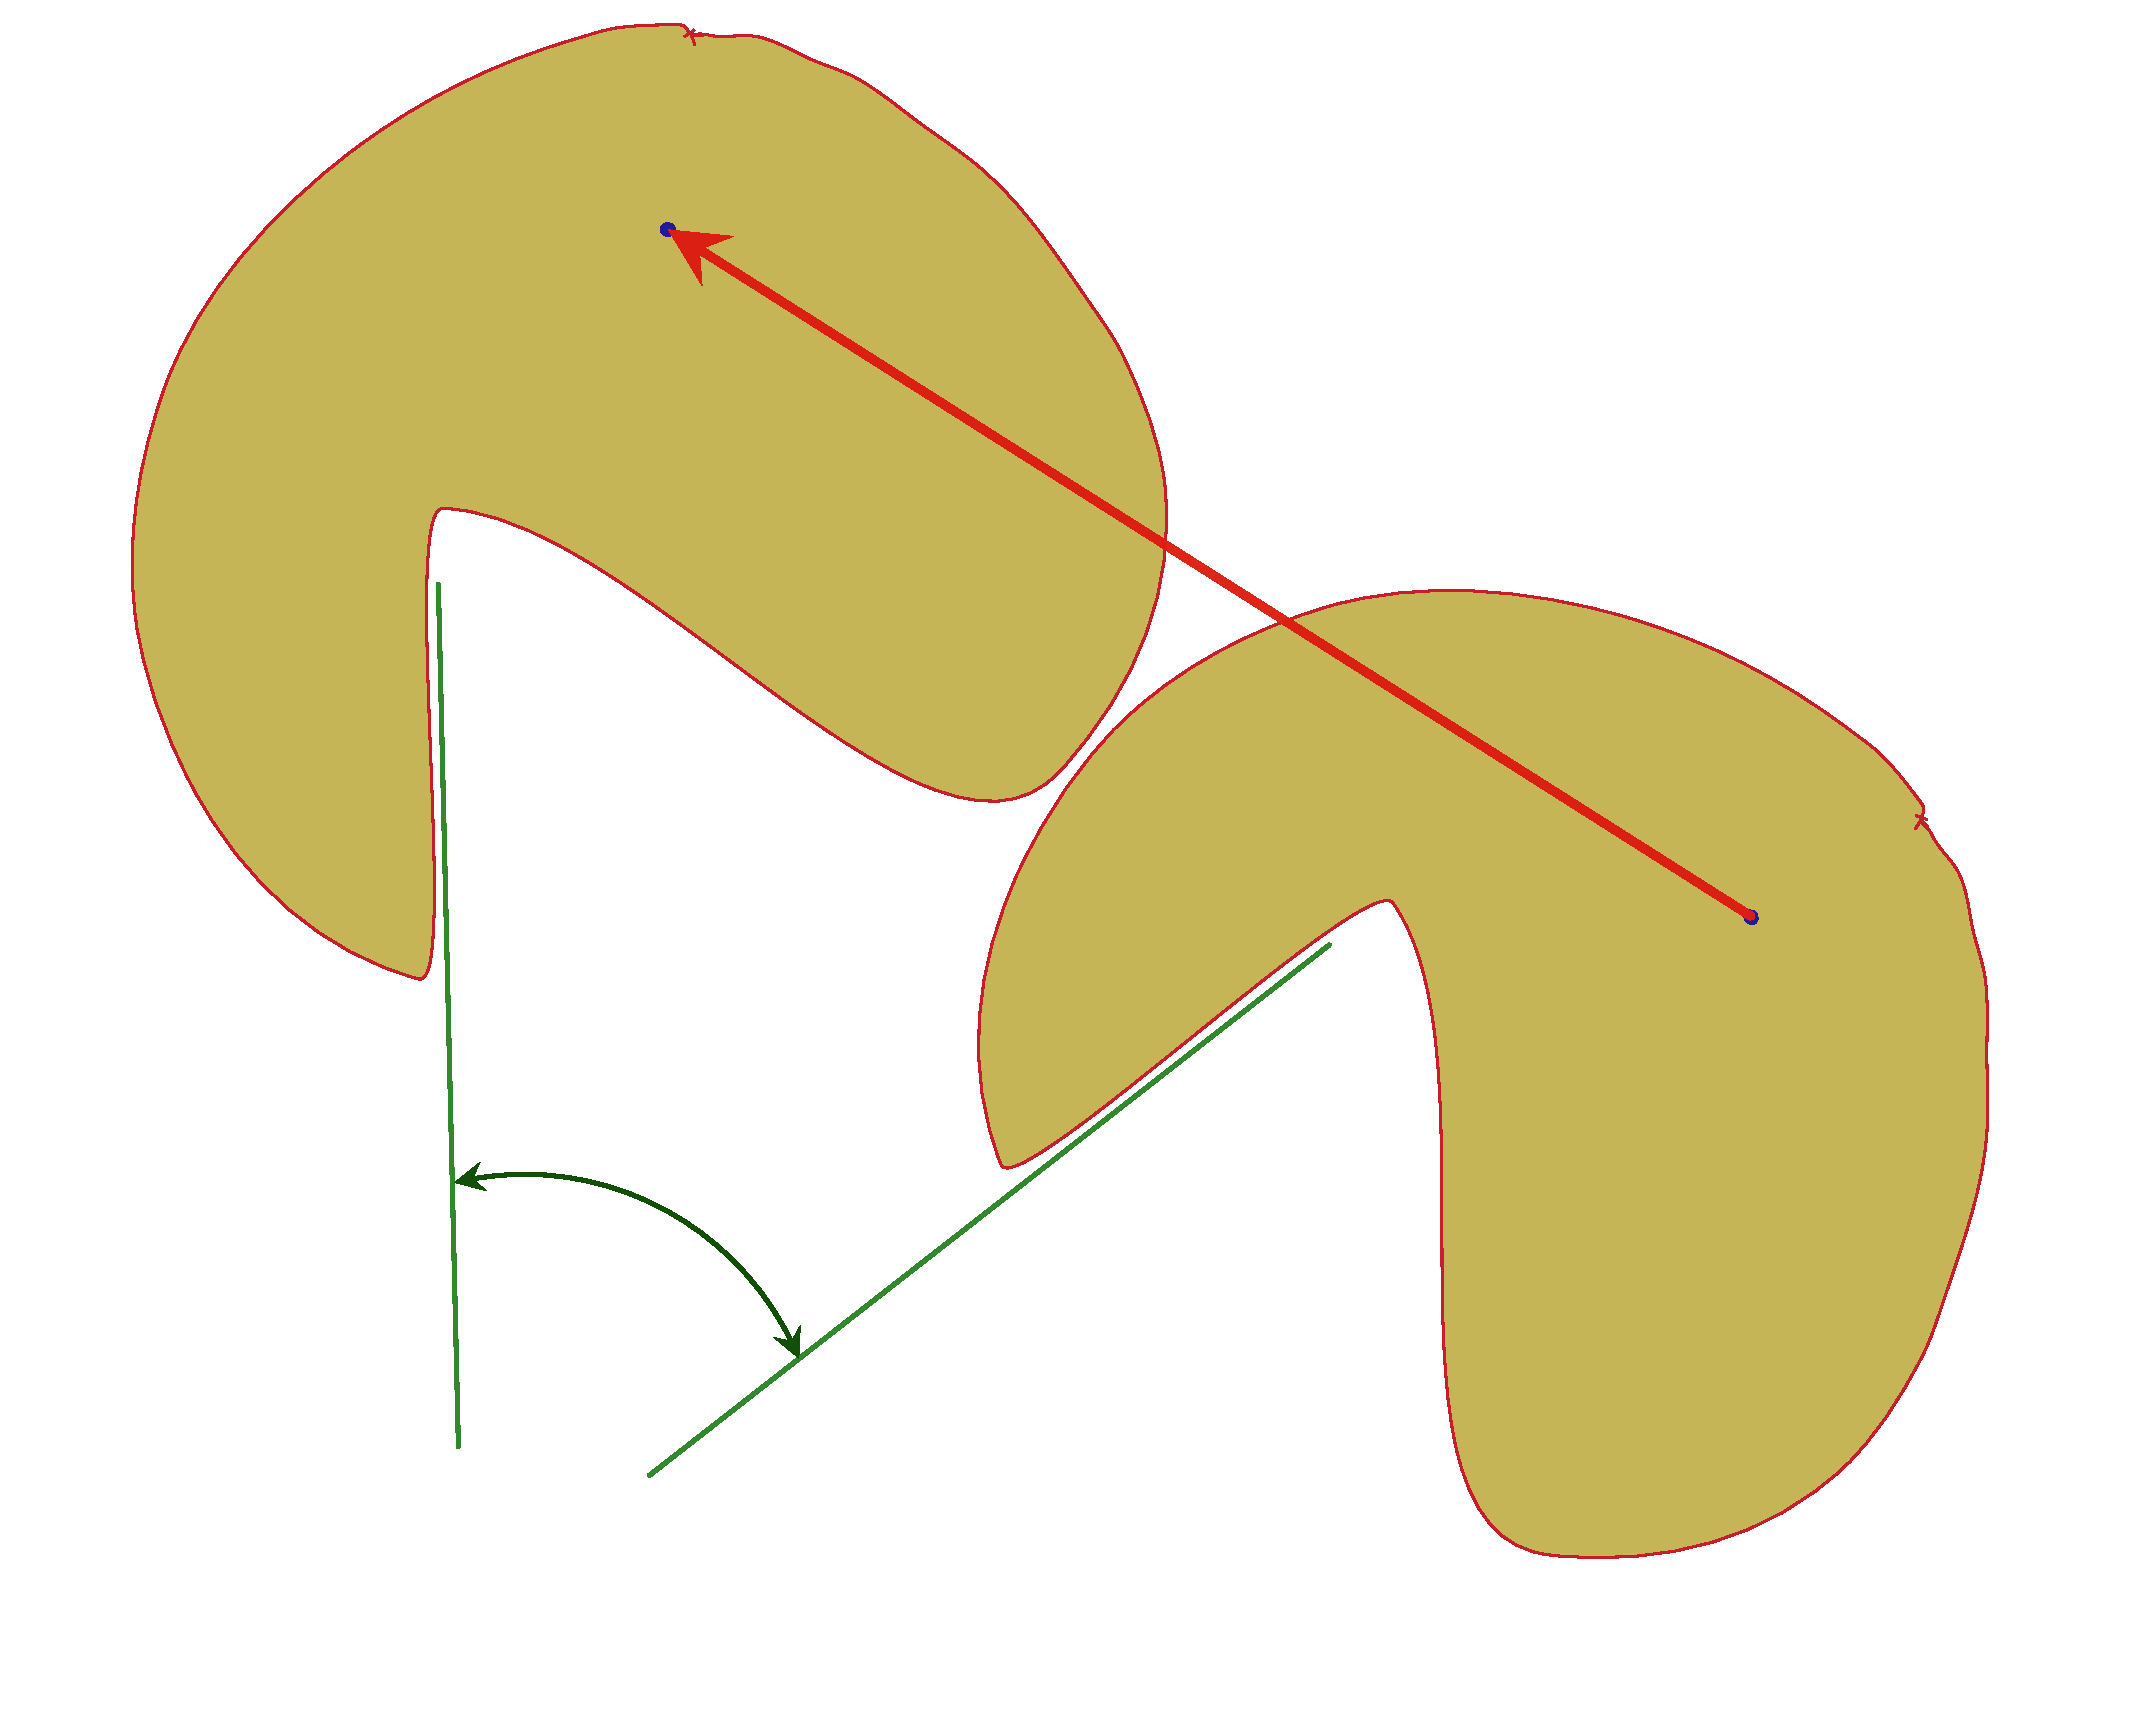
\includegraphics[width=0.42\textwidth]{part1/cinematica/FIG/f12.pdf}
     \end{center}
\begin{picture}(50,0)(-40,0)
\scriptsize{
	\put(31,140){$2)$}
	\put(100,98){$1)$}
\put(12,63){$\Delta \theta$}
\put(-14,98){\bf C}
\put(47,83){\rotatebox{-43}{\bf C}}
\put(53,107){$\Delta{\bm{s}}$}
	\put(4,122){$P_{(2)}$}
	\put(82,73){$P_{(1)}$}
}
\end{picture}
\vskip -7mm
	\caption{\em Spostamento piano di un corpo rigido nel tempo $\Delta t$.}
     \label{fig:f12}
\end{wrapfigure}

\noindent Nella figura \ref{fig:f12} \`e rappresentato lo spostamento {\em piano} del corpo rigido
{\bf C}. Assumiamo che lo spostamento $\Delta{\bm{s}}$,
dalla posizione 1) alla posizione 2), avvenga 
nell'intervallo di tempo $\Delta t$.
Il vettore $\Delta \bm{s}$, che congiunge i punti $P_{(1)}$ e $P_{(2)}$, si chiama
{\em spostamento} \index{spostamento} del punto $P$ nel 
tempo $\Delta t$.
Nello stesso intervallo temporale $\Delta t$ il corpo avr\`a anche mutato orientamento.
Chiamiamo
{\em rotazione} \index{rotazione} $\Delta \theta$ l'angolo compreso
tra una qualsiasi direzione distinguibile sul corpo {\bf C} nella posizione
1) (come pu\`o
essere uno spigolo o un segmento tracciato sul corpo) e lo stesso riferimento,
quando il corpo si trova nella posizione 2).
I rapporti
\begin{equation}
	\lim_{\Delta t \to 0}\;{\Delta {\bm{s}}\over {\Delta t}} = {\bm{v}}\;\;\;\;\;\; \textrm{e}
	\;\;\;\;\;
	\lim_{\Delta t \to 0}\;{{\Delta \theta }\over {\Delta t}} = {\omega}\,, \label{e12}
\end{equation}	
\noindent si chiamano rispettivamente {\em velocit\`a}\index{velocit\`a}
del punto $P$ e {\em velocit\`a angolare}\index{velocit\`a!angolare}
del corpo {\bf C}.
Il lettore con qualche reminiscenza di cinematica
potrebbe chiedersi come mai
non sia stato introdotto alcun {\em sistema di
riferimento}\index{sistema di
riferimento}. 
\`E un fatto che nella maggior parte dei libri moderni di cinematica
si usi spesso riferire gli spostamenti a ``ragionevoli sistemi di riferimento'',
il pi\`u delle volte rappresentati da piccoli {\em assi cartesiani}
disegnati nelle figure nell'angolo in basso a sinistra, come anche a noi accadr\`a di fare pi\`u avanti.
Riteniamo qui superflua la presenza di assi coordinati e, come
abbiamo mostrato, siamo in grado di identificare spostamenti, rotazioni e velocit\`a
senza basarci su di essi.
Ricordiamo per\`o che un sistema di riferimento, almeno implicito, deve
esistere: per noi pu\`o essere la pagina stessa del libro.
A un osservatore (privo di massa) seduto sul corpo {\bf C},  isolato da
tutto il resto dell'universo, sarebbe infatti impossibile rendersi
conto di qualsiasi movimento del corpo stesso.

\begin{figure}[h]
\centering
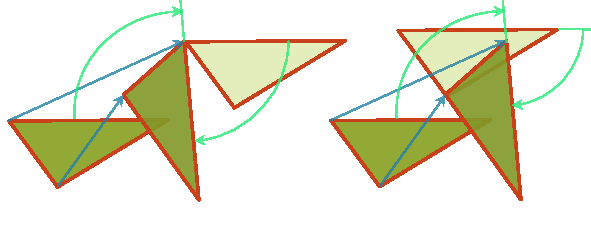
\includegraphics[width=0.9\textwidth]{part1/cinematica/FIG/f13.pdf}
\begin{picture}(0,0)(290,13)
\scriptsize{
\put(14,126){$\Delta \theta$}
\put(64,122){$A'$}
\put(-15,95){${\Delta{\bm s}}_{\scriptscriptstyle{A}}$}
\put(33,88){$B'$}
\put(-37,81){$A$}
\put(106,80){$\Delta \theta$}
\put(15,66){${\Delta{\bm s}}_{\scriptscriptstyle{B}}$}
\color{gray}
\put(56.1,76){$C$}
\color{black}
\put(-14,55){$1)$}
\put(60,55){$2)$}
\put(-9,32){$B$}
\put(70,25){$C'$}
\put(30,15){$a)$}
}
\end{picture}
\begin{picture}(0,0)(117,13)
\scriptsize{
\put(16,131){$\Delta \theta$}
\put(65,116){$A'$}
\put(-15,95){${\Delta{\bm s}}_{\scriptscriptstyle{A}}$}
\put(33,88){$B'$}
\put(-37,81){$A$}
\put(94,89){$\Delta \theta$}
\put(14,66){${\Delta{\bm s}}_{\scriptscriptstyle{B}}$}
\color{gray}
\put(56.3,76){$C$}
\color{black}
\put(-14,55){$1)$}
\put(60,55){$2)$}
\put(-9,32){$B$}
\put(70,25){$C'$}
\put(30,15){$b)$}
}
\end{picture}
	\caption{\em
I due casi riportano la riduzione del medesimo spostamento, sub\`ito
da un corpo rigido,
alla combinazione di due diverse traslazioni con la stessa rotazione
attorno a due diversi poli.
}
\label{fig:f13}
\end{figure}

\section{Teorema di Chasles}\index{Chasles, teorema di}\index{teorema!di Chasles}
La seguente osservazione \`e di importanza fondamentale: lo spostamento
di un corpo {\bf C} \`e inequivocabilmente individuato
dallo spostamento di un qualsiasi suo punto $P$
unitamente alla rotazione dello stesso corpo
{\bf C}. 
Per convincerci di ci\`o consideriamo la 
figura \ref{fig:f13} a) dove il corpo rigido {\bf C} \`e stato sostituito,
per comodit\`a di esposizione,
dal triangolo $\triangle{ABC}$. Il suo spostamento
dalla posizione 1) alla posizione 2), che muove il triangolo $\triangle ABC$
in $\triangle {A'B'C'}$, pu\`o
essere ottenuto mediante la ``somma'' di due successivi spostamenti elementari.

\begin{wrapfigure}{r}{0.42\textwidth}
      \begin{center}
      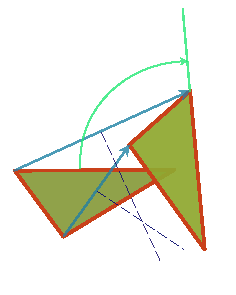
\includegraphics[width=0.35\textwidth]{part1/cinematica/FIG/f14.pdf}
     \end{center}
\begin{picture}(50,0)(-40,0)
\scriptsize{
	\put(0,25){$1)$}
	\put(76,25){$2)$}
\put(17,133){$\Delta \theta$}
%\put(-12,75){\bf C}
%\put(60,100){\rotatebox{-78}{\bf C}}
\put(-28,88){$A$}
\put(63,136){$A'$}
\put(0,48){$B$}
\put(32,105){$B'$}
\put(79,40){$C'$}
\put(40,58){$O$}
\put(47.6,64.2){$.$}
\put(-15,105){$\Delta {\bm s}_{\scriptscriptstyle{A}}$}
\put(1,74.5){$\Delta {\bm s}_{\scriptscriptstyle{B}}$}
}
\end{picture}
\vskip -5mm
	\caption{\em Riduzione generica di uno spostamento piano a una
	rotazione.}
     \label{fig:f14}
\end{wrapfigure}

\noindent Supponiamo dapprima di spostare
il vertice $A$ in $A'$ mediante una {\em traslazione}\index{traslazione}
del triangolo $\triangle{ABC}$, cio\`e mediante uno spostamento che mantenga inalterato
l'orientamento primitivo dei tre lati.  Successivamente ruotiamo il triangolo
attorno al punto $A'$ di un angolo pari a $\Delta \theta$, portandolo a coincidere
col triangolo $\triangle A'B'C'$.
Risulta subito chiaro che la scelta del punto $A$ come base per 
la traslazione del triangolo \`e arbitraria e che in sua vece si sarebbe potuto scegliere $B$, $C$, o qualsiasi
altro punto, dentro o fuori dal perimetro del triangolo, purch\'e legato a muoversi
rigidamente col triangolo stesso. In figura \ref{fig:f13} b) viene rappresentato lo stesso spostamento sub\`ito
dal triangolo $\triangle ABC$ assumendo come base per la traslazione il punto $B$.
Naturalmente, attribuendo 
la traslazione a punti diversi si avranno per essi spostamenti
$\Delta {\bm s}$ diversi, come si evince peraltro dalla figura.
Quando la rotazione $\Delta \theta$ non \`e nulla
\`e possibile
individuare un punto, che potrebbe
non essere incluso nel perimetro del triangolo bens\`i appartenere a un {\em piano mobile}\index{piano mobile}
idealmente incollato su di esso, per il quale lo spostamento $\Delta {\bm{s}}$ \`e nullo.
Tale punto, che indichiamo con $O$, si individua
tracciando dalla mezzeria dei segmenti orientati che
rappresentano gli spostamenti 
{$\Delta {\bm s}_{\scriptscriptstyle{A}}$} e
{$\Delta {\bm s}_{\scriptscriptstyle{B}}$} le loro perpendicolari,
come in figura \ref{fig:f14}: il loro punto di incontro 
\`e il {\em centro dello spostamento rigido piano}.
\`E facile dimostrare (e pertanto lasciato al lettore come esercizio\footnote{
	Si noti che  i due triangoli $\triangle{ABO}$ e $\triangle{A'B'O}$
sono uguali.}) che 
\begin{equation}
	\widehat{AOA'} = \widehat{BOB'} = \widehat{COC'} =\Delta \theta \,.
	\label{e13}
\end{equation}	
\noindent Cos\`i, una rotazione rigida
di un angolo $\Delta \theta$ attorno al punto $O$
porter\`a il triangolo dalla posizione 1) alla posizione 2).
Dalla precedente affermazione si pu\`o dedurre la seguente restrizione
al caso di spostamenti rigidi piani del {\em teorema di 
Chasles}: {\em ogni spostamento rigido piano
si pu\`o ridurre in modo univoco
o a una traslazione o a una rotazione}\footnote{
Ricordiamo questo teorema
come riportato in \cite{finzi}:
``Ogni spostamento rigido, non traslatorio,
si riduce in infiniti modi a uno
spostamento roto-traslatorio, sempre per\`o con la stessa componente di
rotazione. Si riduce poi in modo
univoco a uno spostamento elicoidale''.
Torneremo brevemente nel capitolo \ref{3d}
agli spostamenti tridimensionali, col tentativo
di giustificare, anche in questi casi,
l'esistenza di una direzione principale che \`e l'asse
dell'elica.}.  \label{chasles}

\begin{wrapfigure}{r}{0.54\textwidth}
      \begin{center}
      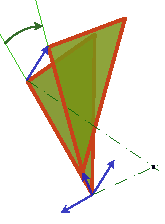
\includegraphics[width=0.35\textwidth]{part1/cinematica/FIG/f15.pdf}
     \end{center}
\begin{picture}(0,0)(-63,1)
\scriptsize{
        \put(-16,178){${\rm d} \theta$}
\put(-17,131){$P$}
\put(40,40){$Q$}
\put(86,61){$O$}
\put(87.5,69.7){$.$}
        \put(-13,153){${\rm d}{\bm s}_{\scriptscriptstyle{P}}$}
        \put(49,77){${\rm d}{\bm s}_{\scriptscriptstyle{P}}$}
        \put(20,54.5){${\rm d}{\bm s}_{\scriptscriptstyle{Q}}$}
        \put(5,26){${\rm d}{\bm \theta} \times \overrightarrow{PQ}$}
}
\end{picture}
        \caption{\em Composizione di spostamenti infinitesimali.}
     \label{fig:f15}
\end{wrapfigure}

\noindent Quanto sin qui riferito circa gli spostamenti piani di un corpo rigido
risulta essere indipendente dalla entit\`a degli spostamenti stessi. Perci\`o le medesime conclusioni resteranno valide anche qualora avessimo a che fare con
spostamenti infinitesimali anzich\'e finiti\footnote{Non \`e vero il contrario: si incorre spesso in errore
trasportando i risultati dedotti considerando spostamenti infinitesimali nel
campo degli spostamenti finiti.}.
Riferendoci alla figura \ref{fig:f15}, possiamo quindi affermare che lo spostamento infinitesimale di un punto $Q$ del triangolo mobile,
{${\rm d} \bm{s}_{\scriptscriptstyle{Q}}$}, 
si possa ottenere sommando lo spostamento infinitesimale
del punto $P$,
{${\rm d} \bm{s}_{\scriptscriptstyle{P}}$}, 
all'effetto che la  rotazione ${\rm d} \theta$, anch'essa infinitesimale,
esercita sul segmento $Q - P$.
E qual \`e questo effetto? Cio\`e: la rotazione ${\rm d} \theta$ applicata
al {\em segmento orientato}\index{segmento orientato} $Q - P$ quale
spostamento produce? Conviene qui fare ricorso
a un ``arnese della matematica'', forse un po' arcigno, 
ma che  risulta troppo comodo
per essere lasciato in disparte: il {\em prodotto vettoriale}\index{prodotto
vettoriale}. Consideriamo quindi la rotazione infinitesimale
${\rm d} \bm{\theta}$\footnote
{
Il vettore ${\rm d} \bm{\theta}$ non \`e, nei casi di moto tridimensionale, il
differenziale di alcun angolo finito di rotazione,
come invece lo \`e nel piano. Rimandiamo
il lettore agli approfondimenti del capitolo \ref{3d} per ulteriori chiarimenti.
}
 come un 
vettore ortogonale al piano dove avviene lo spostamento, senza precisarne
la {\em giacitura}\footnote{Autori importanti, \cite{whittaker} e
\cite{finzi} per esempio, specialmente quando parlano di questo vettore
col senso di velocit\`a angolare (come faremo anche noi tra poco) 
gli  attribuiscono una precisa giacitura, coincidente con
l'{\em asse istantaneo di rotazione}. Ritenendo questa posizione
sterile se non fuorviante, bench\'e non scorretta, preferiamo lasciare tale
vettore
libero di giacere dove vuole.}, col verso dato dalla cosiddetta {\em regola
della mano destra}\index{regola della mano destra} secondo cui il pollice
indica il verso del vettore quando le dita concordano con il senso della
rotazione.
Se al segmento orientato $Q - P$ diamo valore di vettore con 
verso da $P$ a $Q$ si ricava lo spostamento infinitesimale del punto $Q$ come
\begin{equation}
	{\rm d} \bm{s}_{\scriptscriptstyle{Q}} =
	{\rm d} \bm{s}_{\scriptscriptstyle{P}}
	+{\rm d} \bm{\theta} \times \overrightarrow{PQ}\,.
	\label{e14}
\end{equation}	

\vskip 3mm
\noindent Dividendo tutti i termini della \ref{e14} per ${\rm d} t$ otteniamo la seguente 
equazione 

\begin{equation}
	{{ {\rm d} \bm{s}_{\scriptscriptstyle{Q}}}\over{{\rm d} t}} =
	{{ {\rm d} \bm{s}_{\scriptscriptstyle{P}}}\over{{\rm d} t}} +
	{{{\rm d} \bm{\theta}}\over{{\rm d}t}} \times \overrightarrow{PQ}\,,
	\label{e15}
\end{equation}	

\vskip 3mm
\noindent che, con ovvio significato dei simboli, diventa 

\begin{equation}
	{  \bm{v}_{\scriptscriptstyle{Q}}} =
	{  \bm{v}_{\scriptscriptstyle{P}}} +
	{ \bm{\bm \omega}} \times \overrightarrow{PQ}\,.
	\label{e16}
\end{equation}	
\vskip 3mm
\noindent La conoscenza della velocit\`a di un punto e della velocit\`a angolare del corpo,
oppure della velocit\`a angolare e del centro $O$, ci permettono di 
individuare le velocit\`a di tutti i punti del corpo che ne costituiscono il 
suo {\em atto di moto}\index{atto di moto}.
Il centro $O$, nel caso di spostamenti infinitesimali, si chiama
{\em centro istantaneo di rotazione}\index{centro!istantaneo di rotazione} o
{\em centro d'istantanea rotazione}\index{centro!di istantanea rotazione}\footnote{
Se tenessimo traccia delle posizioni via via occupate dal centro d'istantanea
rotazione col procedere del movimento, otterremmo due diverse curve a seconda 
che tale traccia sia lasciata sul piano fisso (il foglio del disegno per
intenderci), oppure sul piano mobile (un piano idealmente incollato col nostro
corpo rigido). Questi due {\em luoghi geometrici} si chiamano rispettivamente
{\em polare fissa}\index{polare!fissa} e {\em polare mobile}\index{polare!mobile}. Esse godono di propriet\`a interessantissime, soprattutto
dal punto di vista della nostra materia, e risultano indispensabili
in alcune analisi cinematiche, come accade nello studio dei profili dei denti
delle ruote dentate. Riteniamo opportuno
rimandare il breve studio che faremo delle polari del moto proprio
al capitolo \ref{cap_ruote_ev},
dove esporremo i principi di progettazione delle ruote dentate.
Segnaliamo agli interessati, che volessero approfondire l'argomento,
 \cite{finzi}, pagg. 168--176
e \cite{sesini1},  pagg. 31--33.}, ed \`e in generale mobile.

\noindent Abbiamo usato la rotazione infinitesimale
${\rm d}{\bm \theta}$ e di conseguenza la velocit\`a angolare $\bm \omega$ come 
vettori ortogonali al piano del moto per i quali il loro {\em prodotto vettoriale} 
con un segmento orientato del piano del moto fornisce uno
spostamento infinitesimale oppure una velocit\`a.

\noindent Vogliamo aggiungere
che la rappresentazione vettoriale delle velocit\`a angolari
non si limita al caso di moti piani, anzi, essa ha origine proprio
nella cinematica dei moti tridimensionali\footnote{Nel caso di moto piano, 
il prodotto vettoriale che coinvolge le rotazioni avviene sempre tra vettori
ortogonali tra loro,
mentre nel caso generale questo non si verifica. Le rotazioni infinitesime
e le velocit\`a
angolari  sono per\`o vettori
particolari. Il loro verso dipende dalla scelta che si fa ``destrorsa''
o ``sinistrorsa'' nella convenzione del prodotto vettoriale e mal
sopportano deformazioni dello spazio che alterino la sua metrica. In pi\`u, la 
possibilit\`a di rappresentare una velocit\`a angolare con un vettore \`e
limitata allo spazio tridimensionale.
},
come esposto in breve nella conclusione del capitolo \ref{3d}.

\chapter{Accelerazioni}

\section{Derivazione della Velocit\`a}

\begin{wrapfigure}{r}{0.43\textwidth}
      \begin{center}
      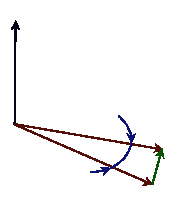
\includegraphics[width=0.3\textwidth]{part1/cinematica/FIG/f16.pdf}
     \end{center}
\begin{picture}(0,0)(-30,-25)
\scriptsize{
	\put(60,32){${\rm d}\theta$}
	\put(5,84){${\rm d}\bm \theta$}
	\put(32,29){$\bm u$}
	\put(35,48){${\bm u}+{\rm d}{\bm u}$}
	\put(93,22){${\rm d}{\bm u}={\rm d}{\bm \theta} \times {\bm u}$}
}
\end{picture}
	\caption{\em Rotazione di un vettore costante.}
     \label{fig:f16}
\end{wrapfigure}
 
L'accelerazione del punto $Q$ di figura \ref{fig:f15} si pu\`o ottenere
derivando la sua velocit\`a rispetto al tempo.
Derivando perci\`o la \ref{e16} otteniamo

\begin{equation}
	{  \bm{a}_{\scriptscriptstyle{Q}}} =
	{  \bm{a}_{\scriptscriptstyle{P}}} +
	\dot{\bm \omega} \times \overrightarrow{PQ}+
	{\bm \omega} \times \dot{{\overrightarrow{PQ}}}\,.
	\label{e17}
\end{equation}

\noindent Concentriamoci sull'ultimo termine
a destra della \ref{e17}: si tratta di eseguire il prodotto
vettoriale tra $\bm \omega$ e il vettore ``derivata rispetto
al tempo di $\overrightarrow{PQ}$''.
Mediante l'ausilio della figura \ref{fig:f16}, la quale vorrebbe essere un
tentativo (forse maldestro) di mostrare il vettore rotazione infinitesimale
${\rm d}{\bm \theta}$ ortogonale al piano dove avvengono gli spostamenti,
affermiamo che la  derivata di un vettore $\bm u$ di modulo costante, come lo \`e anche 
$\overrightarrow{PQ}$,
risulta dalla sola variazione della sua posizione angolare:

\begin{equation}
{{{\rm d}{\bm u}}\over{{\rm d}t}}=
{{\rm d}{\bm \theta} \times 
{\bm u}\over{{\rm d}t}}=
{{\rm d}{\bm \theta}
\over{{\rm d}t}} \times {\bm u}\,.
	\label{e18}
\end{equation}

\noindent Pertanto la \ref{e17} diventa

\begin{equation}
{{\bm a}_{\scriptscriptstyle{Q}}} =
{{\bm a}_{\scriptscriptstyle{P}}} +
\dot{\bm \omega} \times \overrightarrow{PQ}+
{\bm \omega}\times({\bm \omega} \times {{\overrightarrow{PQ}}})\,,
	\label{e19}
\end{equation}
\noindent relazione di grande importanza 
nella cinematica piana\footnote
{
Troveremo di nuovo la \ref{e19} 
e la precedente espressione delle velocit\`a \ref{e16}
nel paragrafo che tratta i {\em moti relativi}. Di fatto queste
espressioni di velocit\`a e accelerazione del punto $Q$ che si ottengono una
volta note la velocit\`a e l'accelerazione di un punto del sistema
mobile, unitamente alla
velocit\`a e all'accelerazione angolari, permettono
il passaggio dalle grandezze cinematiche ``relative'' a quelle ``assolute''.
 Preferiamo per\`o non
mescolare i due problemi, anche se la differenza riguarda la forma e non la sostanza. Per inciso,
le due espressioni citate sopra costituiscono il
{\em teorema di Rivals},\index{Rivals, teorema di}\index{teorema!di Rivals} \cite{sesini1}, pag. 12.
}.	

\begin{wrapfigure}{r}{0.50\textwidth}
      \begin{center}
      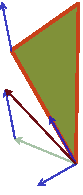
\includegraphics[width=0.25\textwidth]{part1/cinematica/FIG/f17.pdf}
     \end{center}
\begin{picture}(0,0)(-48,-30)
\scriptsize{
\put(6,180){${\bm a}_{\scriptscriptstyle{P}}$}
\put(2,145){$P$}
\put(30,85){${\bm a}_{\scriptscriptstyle{Q}}$}
\put(-3,77){${\bm a}_{\scriptscriptstyle{P}}$}
\put(53,83){${\bm a}_{\scriptscriptstyle{{n}_{Q(P)}}}$}
\put(78,17){$Q$}
\put(41,-2){${\bm a}_{\scriptscriptstyle{{t}_{Q(P)}}}$}
}
\end{picture}
\vskip -7.3mm
	\caption{\em Le componenti dell'accelerazione del punto $Q$.}
     \label{fig:f17}
\end{wrapfigure}
\noindent Il termine
${\bm a}_{\scriptscriptstyle{P}}$
non \`e altro che l'accelerazione del punto $P$.
Il secondo termine,

\begin{equation}
{\bm a}_{\scriptscriptstyle{{t}_{Q(P)}}}=
{\dot{\bm \omega}} \times {{\overrightarrow{PQ}}}\,,
\label{e110}
\end{equation}

\noindent si chiama
{\em accelerazione tangenziale}\index{accelerazione!tangenziale}
del moto di $Q$ attorno a $P$;
il terzo termine,

\begin{equation}
{\bm a}_{\scriptscriptstyle{{n}_{Q(P)}}}=
{\bm \omega}\times({\bm \omega} \times {{\overrightarrow{PQ}}})\,,
\label{e111}
\end{equation}

\noindent  rappresenta l'{\em accelerazione normale}\index{accelerazione!normale}
(a quella tangenziale)
del moto di $Q$ attorno a $P$.
La figura \ref{fig:f17}
dovrebbe chiarire i nomi di questi ultimi due termini.
Tramite la {\em scomposizione del doppio prodotto vettoriale}\index{doppio prodotto vettoriale}\footnote{\label{fig:foot110}
Siano ${\bm u}$, ${\bm v}$, e ${\bm w}$ tre 
vettori in $\mathbb{R}^3$, vale la relazione
\begin{equation}
{\bm u}\times({\bm v}\times{\bm w})=
{\bm v}({\bm u}{\bm w})-
{\bm w}({\bm u}{\bm v})\,.
\label{e2f}
\end{equation}
} 
della \ref{e111} possiamo riscrivere il valore della componente 
normale dell'accelerazione nel modo seguente,
valida nel caso di moti piani
\begin{equation}
{\bm a}_{\scriptscriptstyle{{n}_{Q(P)}}}= -\omega^2 {{\overrightarrow{PQ}}}\,.
\label{e112}
\end{equation}
\noindent La \ref{e19} pu\`o quindi essere
cos\`i riscritta\footnote
{
Ci possiamo
porre la domanda seguente: esiste un punto del piano mobile
con accelerazione nulla?
Uguagliando a zero l'accelerazione
di un generico punto $K$,
dalla \ref{e115}
otteniamo l'equazione

\begin{equation}
{{\bm a}_{\scriptscriptstyle{K}}} = 0 =
{{\bm a}_{\scriptscriptstyle{P}}} +
\dot{\bm \omega} \times \overrightarrow{PK}-
\omega^2 {{\overrightarrow{PK}}}\,,
\label{e1f}
\end{equation}

\noindent che pu\`o essere risolta rispetto al vettore $\overrightarrow{PK}$.
Il punto $K$ cos\`i individuato si chiama {\em centro delle accelerazioni}\index{centro!delle accelerazioni}.
}

\begin{equation}
{{\bm a}_{\scriptscriptstyle{Q}}} =
{{\bm a}_{\scriptscriptstyle{P}}} +
\dot{\bm \omega} \times \overrightarrow{PQ}-
\omega^2 {{\overrightarrow{PQ}}}\,.
	\label{e115}
\end{equation}

\noindent Qualora poi il punto $P$ appartenesse all'asse fisso di rotazione del corpo rigido, 
asse presente in ruote dentate, manovelle,
dischi, volani, ecc.,
la \ref{e115} diventa

\begin{equation}
{{\bm a}_{\scriptscriptstyle{Q}}} =
\dot{\bm \omega} \times \overrightarrow{PQ}-
\omega^2 {{\overrightarrow{PQ}}}\,,
	\label{e116}
\end{equation}

\noindent e i suoi due termini a destra dell'uguale  si chiamano rispettivamente
{\em accelerazione tangenziale}\index{accelerazione!tangenziale}
e {\em accelerazione centripeta}\index{accelerazione!centripeta} del punto $Q$\footnote
{Nel caso in cui il punto $P$ fosse centro d'istantanea rotazione (e non di una rotazione
finita),
la \ref{e116} e i nomi di accelerazione tangenziale e centripeta del punto $Q$ rimarrebbero validi, in quel momento, indipendentemente dall'esistenza o meno
 di un asse fisso di rotazione.
}.

\section{Punto di Vista della Traiettoria}
\noindent Un altro approccio al calcolo dell'accelerazione del punto $Q$ si basa
\begin{wrapfigure}{r}{0.58\textwidth}
      \begin{center}

      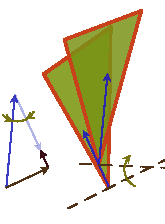
\includegraphics[width=0.45\textwidth]{part1/cinematica/FIG/f18.pdf}
     \end{center}
\begin{picture}(-0,0)(-47,-30)
\scriptsize{
\put(81,22){$Q$}
\put(60,46){$Q'$}
\put(124,58){$O$}
\put(13,80){$-{\bm v}_{\scriptscriptstyle{Q}}$}
\put(51,90){${\bm v}_{\scriptscriptstyle{Q}}$}
\put(-28,75){${\bm v}_{\scriptscriptstyle{Q'}}$}
\put(66,120){${\bm v}_{\scriptscriptstyle{Q'}}$}
\put(-25,105){${\rm d}\theta$}
\put(110,28){${\rm d}\theta$}
\put(124,42){${\rm d}{\bm \theta}$}
\put(-5,30){${\rm d}{\bm v}_{\scriptscriptstyle{Q}_{\scriptscriptstyle{n}}}$}
\put(23,60){${\rm d}{\bm v}_{\scriptscriptstyle{Q}_{\scriptscriptstyle{t}}}$}
}
\end{picture}
\vskip -5.8mm
	\caption{\em Accelerazioni di un corpo rigido: punto di vista intrinseco.}
     \label{fig:f18}
\end{wrapfigure}
sulla valutazione diretta
della derivata di ${{\bm v}_{\scriptscriptstyle{Q}}}$.
\noindent Dopo un tempo infinitesimale ${\rm d}t$ il punto $Q$ si sar\`a portato in $Q'$,
come mostrato nella figura \ref{fig:f18}.
Anche le velocit\`a
${\bm v}_{\scriptscriptstyle{Q}}$ e 
${\bm v}_{\scriptscriptstyle{Q'}}$
saranno in generale diverse 
e possiamo quindi evidenziare la loro differenza infinitesimale.
Con l'aiuto delle figure \ref{fig:f16} e \ref{fig:f18}
abbiamo


\begin{equation}
{\rm d}{\bm v}_{\scriptscriptstyle{Q}_{\scriptscriptstyle{t}}}=
{{\bm v}_{\scriptscriptstyle{Q}}\over{
|{\bm v}_{\scriptscriptstyle{Q}}|}}
\dot{|{\bm v}_{\scriptscriptstyle{Q}}|}{\rm dt}\,,
	\label{e117}
\end{equation}

\begin{equation}
{\rm d}{\bm v}_{\scriptscriptstyle{Q}_{\scriptscriptstyle{n}}}=
 {\rm d}{\bm \theta}\times 
{\bm v}_{\scriptscriptstyle{Q}}\,. 
	\label{e118}
\end{equation}


\noindent Il vettore ${\rm d}{\bm \theta}$ che, come abbiamo
precedentemente chiarito, \`e
ortogonale al piano del disegno, non viene rappresentato in figura se non tramite il proprio simbolo.
A questo punto conviene per\`o introdurre un sistema di
tre versori ortogonali tra loro $\hat{\bm t}$, $\hat{\bm n}$ e $\hat{\bm b}$.
Poniamo il {\em versore tangente}\index{versore!tangente}

\begin{equation}
 \hat{\bm t}= {{{\bm v}_{\scriptscriptstyle{Q}}\over{
|{\bm v}_{\scriptscriptstyle{Q}}|}}}\,,
\label{e119}
\end{equation}

\noindent e imponiamo al {\em versore normale}\index{versore!normale} $\hat{\bm n}$
di essere appunto normale a $\hat{\bm t}$ e al vettore ${\rm d}{\bm \theta}$, inoltre, di essere
diretto come $\overrightarrow{QO}$;
infine imponiamo a $\hat{\bm b}$, chiamato
{\em versore binormale}\index{versore!binormale},
di avere la medesima direzione e il medesimo verso di ${\rm d}{\bm \theta}$.
\noindent Le relazioni \ref{e117} e \ref{e118} si possono ora scrivere, aiutandoci con
i versori della {\em terna intrinseca}\index{terna!intrinseca} test\'e introdotta,
nel seguente modo:
\begin{equation}
{\rm d}{\bm v}_{\scriptscriptstyle{Q}_{\scriptscriptstyle{t}}} = {\hat{\bm t}}
\dot{|{\bm v}_{\scriptscriptstyle{Q}}|}{\rm d t}\,,
	\label{e120}
\end{equation}
\begin{equation}
{\rm d}{\bm v}_{\scriptscriptstyle{Q}_{\scriptscriptstyle{n}}} =
{\rm d}{\theta}
({\hat{{\bm b}}}\times 
{\bm v}_{\scriptscriptstyle{Q}})\,. 
	\label{e121}
\end{equation}
\noindent L'angolo ${\rm d}\theta$ si pu\`o ottenere dal rapporto tra arco
$|(Q'-Q)|=|{\bm v}_{\scriptscriptstyle{Q}}|{\rm d}t$
e il {\em raggio di curvatura della traiettoria}, individuato da $\rho=|(O-Q)|$ o alternativamente
da $\rho=|(O-Q')|$, cio\`e
\begin{equation}
{\rm d}{\theta}=
{|{\bm v}_{\scriptscriptstyle{Q}}|{\rm d}t 
\over{\rho}}\,.
\label{e122}
\end{equation}
\noindent Dividendo tutte le espressioni per ${\rm d}t$ e sostituendo ${\rm d}{\theta}$ con l'espressione fornita dalla
\ref{e122}, le \ref{e120} e \ref{e121} diventano
\begin{equation}
{\bm a}_{\scriptscriptstyle{Q}_{\scriptscriptstyle{t}}}=
{\hat{\bm t}}
\dot{|{\bm v}_{\scriptscriptstyle{Q}}|}\,,
	\label{e123}
\end{equation}
\begin{equation}
{\bm a}_{\scriptscriptstyle{Q}_{\scriptscriptstyle{n}}}=
{|{\bm v}_{\scriptscriptstyle{Q}}| 
\over{\rho}}
({\hat{{\bm b}}}\times 
{\bm v}_{\scriptscriptstyle{Q}})\,. 
	\label{e124}
\end{equation}
\noindent Ma il versore 
${\hat{\bm b}}$, che \`e concorde a ${{\rm d}\bm \theta}$ sia come direzione sia come verso,
risulta ortogonale a ${\bm v}_{\scriptscriptstyle{Q}}$ e al versore
${\hat{\bm n}}$, pertanto 
\begin{equation}
({\hat{{\bm b}}}\times 
{\bm v}_{\scriptscriptstyle{Q}})= 
{\hat{\bm n}}
|{\bm v}_{\scriptscriptstyle{Q}}|\,,
	\label{e125}
\end{equation}
\noindent e la \ref{e124} si pu\`o scrivere nel modo seguente
\begin{equation}
{\bm a}_{\scriptscriptstyle{Q}_{\scriptscriptstyle{n}}}=
{\hat{\bm n}}
{|{\bm v}_{\scriptscriptstyle{Q}}|^2 
\over{\rho}}\,.
	\label{e126}
\end{equation}
\noindent Riassumendo, abbiamo per la accelerazione del punto $Q$
\begin{equation}
{{\bm a}_{\scriptscriptstyle{Q}}} =
{\hat{\bm t}}
\dot{|{\bm v}_{\scriptscriptstyle{Q}}|}+
{\hat{\bm n}}
{|{\bm v}_{\scriptscriptstyle{Q}}|^2 
\over{\rho}}\,.
	\label{e127}
\end{equation}
\noindent Ci si pu\`o chiedere quale sia la differenza tra l'espressione \ref{e115},
ottenuta poc'anzi, e la formula alternativa \ref{e127}.
Si nota immediatamente che le informazioni necessarie
all'individuazione dell'accelerazione del punto $Q$, mediante i due approcci,
sono diverse.
Da una parte l'espressione \ref{e115} richiede di sapere l'accelerazione del
punto $P$, unitamente alla velocit\`a e all'accelerazione angolari del corpo
rigido, nonch\'e la posizione di $Q$ rispetto a $P$.
Dall'altra dobbiamo sapere cosa succede alla velocit\`a del punto $Q$ in due
posizioni temporali infinitamente vicine, il che equivale a conoscere anche
la geometria della {\em traiettoria}\index{traiettoria} del punto $Q$. 
L'espressione \ref{e126} risulta molto comoda qualora si conoscano la
velocit\`a e la {\em curvatura della traiettoria}\index{curvatura!della traiettoria} percorsa da $Q$. 
Immaginiamo di percorrere con un'automobile una curva e di trovarci in un
punto dove il suo raggio, in generale variabile, sia noto\footnote
{
Non \`e facile avere a disposizione una tale informazione,
anche se forse si potrebbe 
ottenere dalle mappe, oggigiorno disponibili su vari dispositivi.
}
e di conoscere la nostra velocit\`a
(il suo modulo) mediante la lettura del tachimetro: ecco che tramite la \ref{e126}
risulta immediato calcolare la nostra accelerazione centripeta.
Inoltre, la \ref{e127} \`e equivalente alla \ref{e116}
 (il lettore pu\`o verificarlo tramite
le relazioni che intercorrono tra le varie quantit\`a) quando il moto ha un asse fisso.
Vale la pena aggiungere che la \ref{e127}
\`e stata ricavata senza 
fare uso della planarit\`a del moto, quindi la sua validit\`a si estende
anche ai moti tridimensionali.
\newpage
\thispagestyle{empty}
\null

\endinput 


